    
\tikzstyle{feuille}=[ draw, rectangle, inner sep = 0.12cm]
\tikzstyle{noeud}=[ draw, rectangle,rounded corners, minimum width= 0.64cm, line width = 1pt]
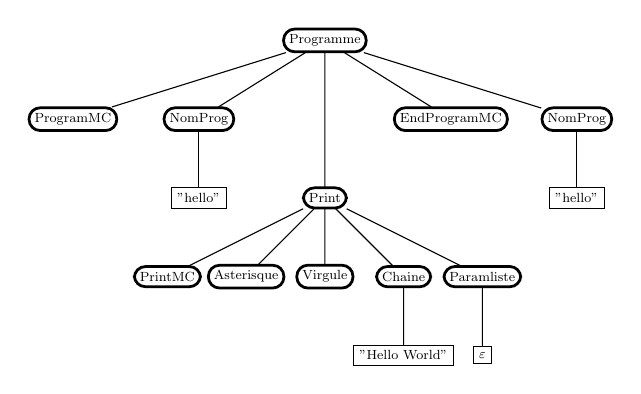
\begin{tikzpicture}[
        baseline=(base), 
        level/.style={sibling distance = 1.6cm/#1, level distance = 1cm},
        every node/.style={scale=0.6, font=\footnotesize}
    ]
    
    \node[ noeud] {Programme}
    child { 
        node[noeud] (base) {ProgramMC}
    }
    child {
        node[noeud] {NomProg}
        child {node[feuille] {"hello"}}
    }
    child [ level distance=2cm]{ 
        node [ noeud] {Print}
        child [sibling distance= 1cm] {
            node [noeud] {PrintMC}
        }
        child [sibling distance= 1cm]{
            node [noeud] {Asterisque}
        }
        child [sibling distance= 1cm]{
            node [noeud] {Virgule}
        }
        child [sibling distance= 1cm]{
            node [noeud] {Chaine}
            child { 
                node [feuille] {"Hello World"}
            }
        }
        child [sibling distance= 1cm] {
            node [noeud] {Paramliste}
            child { 
                node [feuille] {$\varepsilon$}
            }
        }
    }
    child { 
        node[ noeud] {EndProgramMC}
    }
    child {
        node[noeud] {NomProg}
        child {node[feuille] {"hello"}}
    };

\end{tikzpicture}